\documentclass[14pt,oneside,final]{vlsithesis}
\title{Security-Aware RWA for Dynamic Traffic Using Path Protection In WDM Networks}
\author{Kamaljeet Singh Gill}
\degree{Master of Science}
\doctype{Thesis}
\dept{School of Computer Science}
\numberofmembers{4}

\membera{E. Raheem}
\depta{Department of Electrical and Computer Engineering}
\memberb{D. Wu}
\deptb{School of Computer Science}
\memberc{A. Jaekel, Advisor}
\deptc{School of Computer Science}
\memberd{S. Bandyopadhyay, Co-Advisor}
\deptd{School of Computer Science}

\defenseyear{2018}
\defensedate{January 17, 2018}


\usepackage{comment, graphicx}
%\usepackage{tabularx}\textbf{}
\usepackage{algorithm}
%\usepackage{algpseudocode}-
%\usepackage{graphicx, comment, fullpage, algorithm}
\usepackage{graphicx, algorithm}
\usepackage{url, hyperref}
\usepackage{chngcntr}
\counterwithin{table}{chapter}


%%%%%%%%%%%%%%%%%%%%%commenting out all packages%%%%%%%
%\begin{comment}
%\documentclass{article}
\usepackage{graphicx, hyperref}
%\usepackage{amsthm}\leftrightarrow
\usepackage{amsmath}

\usepackage{cite}
%\usepackage{natbib}
\usepackage{amssymb}
%\usepackage{mathrsfs}
%\usepackage{comment}
\newtheorem{mydef}{Definition}
\newtheorem{theorem}{Theorem}
%\newtheorem{lemma}{Lemma}
\usepackage{tabularx}
%\usepackage{subfigure}
\usepackage{algorithm}
\usepackage{algpseudocode}
%\usepackage{lscape}
%\usepackage{rotating}
%\usepackage{hyperref}
%\usepackage{fullpage}
\usepackage{setspace}
\usepackage{caption}

\doublespacing


%\usepackage{breqn}


%%%%%%%Kaushik%%%%%%%%%%%%%%%%%%%%%%%%
\usepackage{graphicx}              % to include figures
\usepackage{float}
\usepackage{caption}
%\usepackage{subcaption}
\usepackage{amsmath}               % great math stuff
\usepackage{amsfonts}              % for blackboard bold, etc
%\usepackage{amsthm}                % better theorem environments
\usepackage{algorithm}
%\usepackage[noend]{algpseudocode}
%\part{%%%%%%%Kaushik%%%%%%%%%%%%%%%%%%%%%%%%}
\usepackage{graphicx}              % to include figures
\usepackage{float}
\usepackage{caption}
%\usepackage{subcaption}
\usepackage{amsmath}               % great math stuff
\usepackage{amsfonts}              % for blackboard bold, etc
%\usepackage{amsthm}                % better theorem environments
\usepackage{algorithm}
%\usepackage[noend]{algpseudocode}
\usepackage{longtable}
\usepackage{multirow}
\usepackage[titletoc,title]{appendix}
\counterwithin{figure}{chapter}

\begin{document}

\maketitle
\makeapproval
\pagenumbering{Roman}
\setcounter{page}{3}

\makedeclaration

\abstract{
	 Security and attack management have become the prime concern for the network operators due to high data transfer rates and vulnerabilities associated with transparency in WDM networks. In the recent years, there is a substantial increase in perception to develop suitable mechanisms for subduing the adverse effects of malicious attacks such as high power jamming and tapping attacks.In transparent optical networks (TONs) traffic is carried over the optical fibers in the form of signals called lightpaths, creating a virtual topology over the physical interconnections of an optical fiber. This allows an exchange of an enormous amount of data at a very high speed. A fault or an attack on the network can lead to data tampering and data loss. Unlike faults, malicious attacks may not be localized and we cannot handle them with the standard fault-tolerance mechanisms in WDM networks.
	 
The Routing and Wavelength Assignment (RWA) problem assigns appropriate routes and wavelengths to all associated lightpaths in the network. Most the researchers considered the static traffic model, where the network requests (i.e. lightpaths to be established) are known in advance and last over long durations. In this thesis, we are solving the security-aware problem for dynamic requests by using protection strategy known as dedicated path protection (DPP). In the dynamic model, lightpaths are generated on-demand, and RWA must be performed based on available resources that are not being used by ongoing lightpaths. We propose an Integer linear programming (ILP) formulation to maximize requests satisfaction and reducing the disruption in the network due to malicious attacks (In-band and out-band).
	
	\nocite{*}
}

%\dedication{}


\dedication{
			\centerline	{$To\ my\ loving\ family:$}
			
			\centerline {$Grandmother:$ $Surinder\ Kaur$}
			\centerline {$Father:$ $Balvinder\ Singh\ Gill$}
			\centerline {$Mother:$ $Sukhpal\ Kaur$}
			\centerline {$Brother:$ $Jujhar\ Singh\ Gill$}}

\acknowledgements{
	I would like to express my sincere gratitude to my supervisor Dr. Arunita Jaekel, without him my thesis and my whole Master's is incomplete. I also offer my sincere appreciation to my co-supervisor Dr. Subir Bandyopadhyay for his continuous support.
	
	Secondly, I would also like to express my gratitude to my committee members Dr. Esam Abdel-Raheem, and Dr. Dan Wu for their beneficial advice and suggestions for my thesis.
	

	
}


\tableofcontents
\listoffigures
\listoftables


\mainmatter
\chapter{Introduction}

\section{Overview}

The Internet is the global system of interconnected computer networks that use the Internet protocol suite (TCP/IP) to link devices worldwide. It is a network of networks that consists of private, public, academic, business, and government networks of local to global scope, linked by a broad array of electronic, wireless, and optical networking technologies. The Internet carries a vast range of information resources and services, such as the inter-linked hypertext documents and applications of the World Wide Web (WWW), electronic mail, telephony, and file sharing.. A remarkable growth of internet traffic has been observed between the years 2000 to 2015, calculated around 832.5\% \cite{wiki:IN} . There is an urgent need of communication mechanisms, which can help the users to access large amounts of data at high speeds and also to improve the reliability of data transfers. Optical networks provide the ideal infrastructure to handle this enormous growth \cite{wiki:IN}.

Optical networks consist of optical fibers, which use signals encoded in the form of light to transmit the information to various nodes into the network. Optical communication provides robust, large capacity, high transmission rates over long distances with high-reliability transmission, interconnection, and management for the multi-node networks. There are certain components on which optical networks rely, e.g. optical amplifiers, lasers, LEDs, multiplexer, demultiplexer, optical switch, and wavelength division multiplexing (WDM) technology.

Security is a major concern in communication systems. Furthermore, there are some vulnerabilities associated with transparency in all-optical networks. Physical layer attacks caused by the high-powered jamming signals can lead to data tampering and can even result in loss of data.
Techniques to reduce and limit the impact of such attacks are an important research problem. In this thesis, we propose an attack-aware routing and wavelength assignment (RWA) formulation to allocate resources in a ‘safe’ way to incoming communication requests.



\section{Motivation}

Transparent optical networks (TONs) are capable of accommodating with the rapid increase and growing future traffic requirements. Transparency in the optical networks leads to the high data communication without undergoing the opto-electro conversion. One of the main advantages of the optical networks over the metal communication networks is security. Still, there are several vulnerabilities aspects associated with distinct devices used in the optical fiber technology that can lead to the attacks by exploiting non- linearities such as crosstalk (in-band or out-of-band). It is possible take advantages of these vulnerabilities and can carry out multiple attacks, breaching the network acquiring an unauthorized access to the information flowing through the optical fiber, which will compromise some key aspects of network and information security (confidentiality, integrity, availability, non- repudiation network, and information security).
Some of the following recent attack attempts have been made on the optical networks to gain unauthorized access to the data signals.

\begin{enumerate}
	\item In 2003, ” Tapping a fiber optic cable without being detected, and making sense of the information you collect certainly isn'��t trivial, but has been done for the past seven or eight years”- \cite{wiki:AA}
	\item Eavesdropping case was reported in March 2003, “The Wolf Report”, Security officials in the US discovered an illegally installed fiber eavesdropping device in Verizon’s optical network. It was placed at a mutual fund company….shortly before the release of their quarterly numbers \cite{wiki:AA}.
	\item On April 6, 2003, an illegal attempt was made to access the information from the optical network in Baghdad- Fox News \cite{wiki:AA}.
	\item In 2005, Kimberllie Witcher noted in his research paper published by the SANS Institute, that industry experts feel that it is as easy to hack a fiber optic cable as a copper cable \cite{wiki:CA}. 
	\item On 22nd June 2015, Pierluigi Paganini has written an article about Kevin Mitnick hacking an optical fiber data cable just by using an optical fiber clip-on coupler \cite{wiki:CA}.
\end{enumerate}

This demonstrates how the attackers can take advantage of the vulnerabilities and security threats related to the optical fiber networks. With the constant development in the technology, equipment to breach the security of the networks are becoming easily affordable and compact each day. Hence, there is need to develop a technology to handle this kind of attacks on the optical fiber networks to provide the user a secure and robust communication.

\section{Solution Outline}

In this thesis, we propose an integer linear program (ILP) formulation approach to address the attack-aware RWA problem for dynamic traffic model, using dedicated path protection (DPP) \cite{el2015attack} in WDM optical network. A physical network is given, which consists of the nodes and edges. Each edge is considered to be bidirectional, and is implemented by a pair of optical fibers, each carrying traffic in one direction.


The RWA problem searches for the physical paths and available wavelengths, for routing communication requests. In this thesis, we are considering both in-band and out-of-band attacks, which will be explained in detail in Chapter 2. The main objective of the ILP formulation is to maximize the number of requests that can be established in the network, by carrying out AA-RWA (attack-aware RWA) for each request. Numerous simulation scenarios considering the different network topologies, demand sets, etc. are carried out to evaluate the performance of the proposed approach.


\section{Thesis Organization}

The thesis is organized as follows: In chapter 2 an outline of different optical networking components and fundamental concepts of WDM optical networks is presented, as well a review of previous work on attack aware RWA in optical networks. Chapter 3 describes our proposed attack aware ILP for dynamic traffic using dedicated path protection (DPP). In chapter 4, simulation results for the proposed ILP for different standard topologies are discussed and analyzed. Finally, our conclusions, and some directions for future work are presented in chapter 5.



\chapter{Review of Optical Fiber Networks}

Communication industry, undergoing a change of communication medium i.e., to fiber optic networks since its invention in early 1970’s. This communication has become the integral part of world’s communication technology because of its capability of carrying data (tera bits per second) at high volume and speed by connecting different continents. Optical fiber shows a remarkable decrease in signal attenuation, distortion, cost and increase in bandwidth capabilities.\cite{wang2002partial}\cite{ramaswami2009optical}\cite{furdek2012physical}


\begin{figure}[h!]
	\centering
	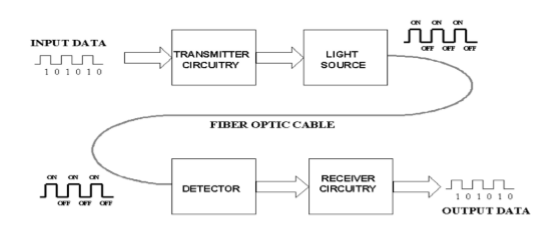
\includegraphics[scale= 1.0]{img/architecture.png}
	\caption{{\em Architecture of optical networks}}
	%	\label{triangleQG}
\end{figure}

Figure [2.1] shows the basic architecture of an optical fiber network. There are multiple components are used for opto-fiber communication\cite{zang2000review}. Transmitter and receiver are used to convert electrical signals to optical signals and vice versa, mostly at the end nodes. Sometimes it is necessary to amplify the signal to strength them. In all-optical networks, also called transparent optical networks (TONs), there is no optical-electrical-optical (OEO) conversion at intermediate nodes.

\section{Optical Components}

In this section, we describe some of the main components used in optical networks.
Optical Fiber

\begin{figure}[h!]
	\centering
	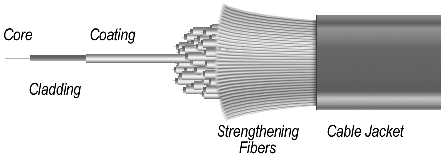
\includegraphics[scale= 0.7]{img/opticalFiber.png}
	\caption{{\em Basic structure of an optical fiber}}
	%	\label{triangleQG}
\end{figure}

An optical fiber is a thin glass strand which runs through the core of the cable carrying the signals in the light pulses. The light pulse is injected into the strand from one end of the optical fiber reaches to the other end with high speed and low transmission loss. The basic structure of the optical fiber consists of core, which carries actual light signal, surrounded by cladding, a layer of glass with lower refractive index than the core which is necessary for the phenomenon called $total\ internal\ reflection$ \cite{wiki:TIR}, protective buffer coating and strengthening fibers followed by the generic cable jacket, acts as two protective layers which are shown in the figure [2.2]. While, the light signal is injected into the core signal remain in the core throughout traversing from source to destination leads to total internal reflection inside the cable.


Optical fibers are further classified into two major categories:

\begin{itemize}
	\item $Single mode cable$
	\item $Multimode cable$
\end{itemize}

Single mode cable consists of a single thread-like glass strand running through the core of the cable with a diameter of 8.3 to 10 microns \cite{wiki:SM}. It generally carries bandwidth higher than the multimode fiber. Single mode fiber is basically used in the application which are required to carry multiple wavelengths with same mode so only single cable is needed. Technically, in single mode we have multiple wavelengths of light are used with same set of nodes having higher transmission rate and can carry data 50 times more than multimode, and one drawback is high cost. In single mode fiber it has much smaller core than multimode providing an advantage of no distortion because of the small core and single ray of light propagating through the core (signal degradation caused by light propagation of different frequencies at different speeds) that could result from overlapping of light pulses and provides the least signal attenuation (referred as loss of signal intensity)\cite{chu2005dynamic}.


Multimode cable consist of a bit larger core diameter ranging between 50 to 100 micron, which is larger than single mode fiber \cite{wiki:MM}.  It provides high bandwidth at high speeds over medium distances, such as within a confined area like buildings, campus providing data transfer speeds ranging from 10 Mbit/s to 10 Gbit/s over the link lengths upto 600 meters (2000 feet )\cite{mukherjee2006optical}. Architects have switched to single mode fiber in new applications using bandwidth in Gigabit and higher, due to multiple rays of light, signal distortion occurs at the receiving end, results in an unclear and incomplete data transfer in long distance cables\cite{anand2001static}.


\section{Optical network components}


In this section, a brief description of optical network components that are discussed in this thesis is provided. The vulnerabilities associated with different optical networking components lead to crosstalk during optical transmission \cite{furdek2011physical}. These vulnerabilities can be exploited by the attacker to initiate an attack.



\subsection{Optical Multiplexer (MUX): }

Optical multiplexer is a device use to combine different wavelengths of light carrying signals onto an optical fiber. It receives optical signals from several channels to merge and couple them into one optical fiber \cite{wiki:AD}


\subsection{Optical Demultiplexer (DEMUX):}

Optical demultiplexer is a reverse multiplexer use to split the combined modulated signal onto the different channels carrying signals \cite{wiki:AD}.

\begin{figure}[h!]
	\centering
	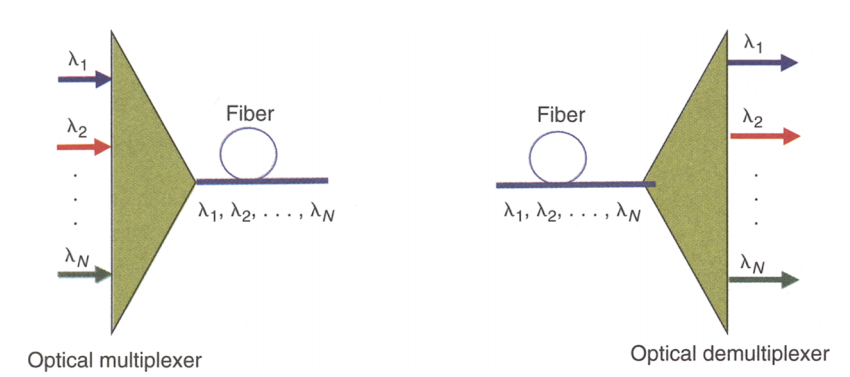
\includegraphics[scale= 0.6]{img/Multiplexer.png}
	\caption{{\em Multiplexer and demultiplexer}}
	%	\label{triangleQG}
\end{figure}


\subsection{Optical add or drop multiplexer (OADM):}

The optical add or drop multiplexer is a combined version of multiplexer and demultiplexer, which selectively drops one or more channels carrying optical signals leaving the channel empty. The OADM uses that empty channel and allocates it to another incoming optical signal carrying data in the same direction of flow. These devices are further divided into two categories namely, fixed or dynamic. The wavelength selection is static in these devices, between the optical DEMUX/MUX. In the dynamic OADMs, the wavelength selection is reconfigurable. These devices can only handle simple networks like ring and linear topologies, where traffic load is less.


\begin{figure}[h!]
	\centering
	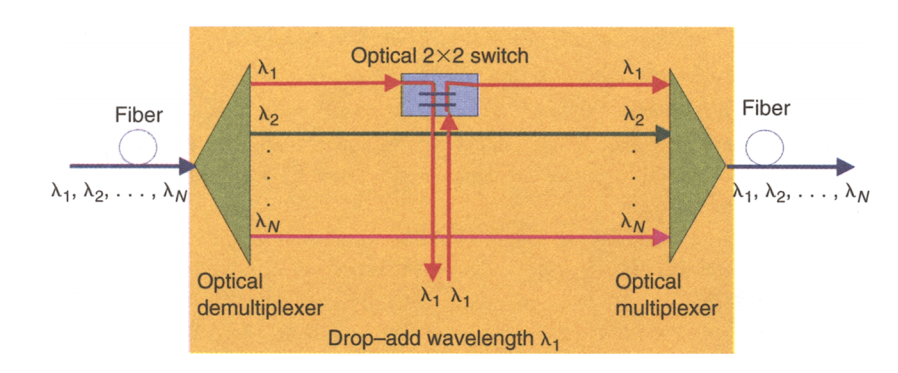
\includegraphics[scale= 0.6]{img/adddrop.png}
	\caption{{\em Add drop explanation}}
	%	\label{triangleQG}
\end{figure}


\subsection{Optical cross connect switch (OXC):}

The OXCs are another type of optical networking device, which connect optical signals between the output of DEMUX and the inputs of MUX in a single node. An OXC’s structure normally consist of MUX’s, DEMUX’s and optical switching fiber [7]. Routes through the switching fiber can be determined in two possible ways: static and dynamic. In the static cross connect switch, the connections between the respective DEMUXs and MUXs are fixed. In dynamic OXC, it is possible to modify the routing of signals according to the requirement. As the switch ports are closely connected, it is possible for the device to turn out to be a source of in-band crosstalk, where the signals of same wavelength interact with each other.


\begin{figure}[h!]
	\centering
	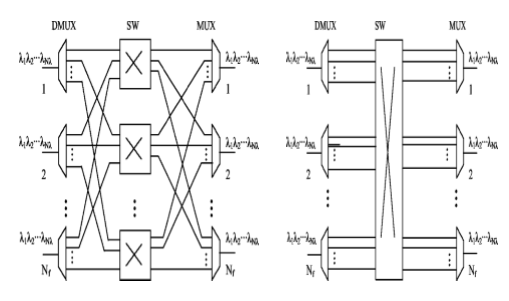
\includegraphics[scale= 0.9]{img/OXC.png}
	\caption{{\em (a) Static and (b) Dynamic Optical Cross Connect Switch}}
	%	\label{triangleQG}
\end{figure}


\section{Basic Concepts}


\subsection{Wavelength Division Multiplexing (WDM)}


An optical fiber can handle a very large amount of data, around 50 terabits per second \cite{wiki:WDM}. Existing electronic devices that can be connected to the optical network cannot receive and transmit data at such highspeed. To overcome this bottleneck, a new technique was introduced called wavelength division multiplexing, defined as: “wavelength division multiplexing (WDM)\cite{dutta2002traffic}, is the idea of merging or multiplexing a number of optical carrier wavelengths or signals onto a modulation signal on a single fiber using channels traversed with different wavelength formats of light.” \cite{wiki:WDM}


In WDM networks, the bandwidth of a network is divided into multiple non-overlapping ranges of frequencies called channels, where each channel corresponds to a different carrier wavelength and is capable of sending data independently. The wavelength division multiplexing method merges the data incoming from different devices using different wavelengths and transmits them over single optical fiber, and after traversing through the optical fiber at the receiving end, the wavelength division multiplexing method splits the signals based on different carrier wavelengths and routes them to their appropriate destinations \cite{tripathi2007reduction}.


When an optical signal traverse through the optical fiber, the signal quality and strength degrades. It degrades in terms of amplitude, error bit rate, shape, and phase. To overcome signal deterioration limitation amplifiers are used in the network.

A single mode optical fiber cable has a very low loss transmission with an enormous bandwidth (tens of terahertz) that no existing opto-electronic sender or receiver device can handle. Wavelength Division Multiplexing (WDM) addresses these problems by dividing the bandwidth into several low speed channels (10 Gbits/s to 100 Gbits/s) and reaching a high total data rate by combing several channels \cite{nizampatnam2017minimizing}


\begin{figure}[h!]
	\centering
	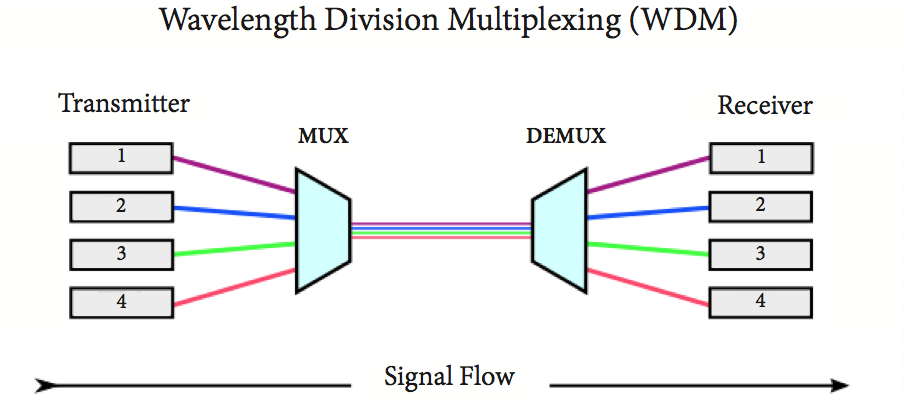
\includegraphics[scale= 0.5]{img/wdm.png}
	\caption{{\em Wavelength Division Multiplexing}}
	%	\label{triangleQG}
\end{figure}


In the Figure [2.6], optical signals on individual channels (colors: purple, blue, green and pink) are sent from respective transmitters (1 - 4) to be multiplexed and traverse on a single optical fiber cable. And, at the receiver's end they are demultiplexed and sent to respective receivers (5 - 8) to reach their appropriate destinations.

\subsection{ Routing And Wavelength Assignment (RWA)}

The physical topology of an optical network consists of the set of nodes and the fiber links that interconnect these nodes, as shown below in Figure [2.7]. A lightpath is an all-optical connection established between two end nodes in the physical topology, where the signal remains in the optical domain. A lightpath is unidirectional, connecting a source node to a destination node, and can traverse multiple links in the physical topology. Figure [2.7] shows four lightpaths established over the given physical topology. In the network, each lightpath is assigned a particular route and carrier wavelength.

\begin{figure}[h!]
	\centering
	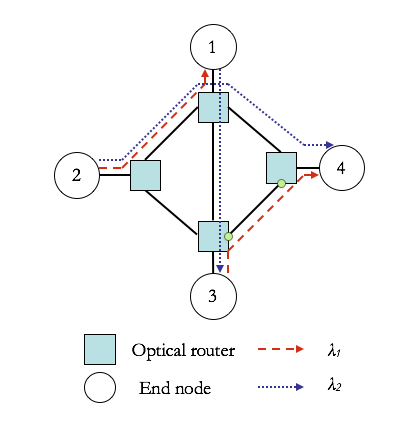
\includegraphics[scale= 0.6]{img/topology.png}
	\caption{{\em Physical and Logical Topology}}
	%	\label{triangleQG}
\end{figure}

The Routing and Wavelength assignment(RWA) problem is the act of establishment of an effective route and assigning an available wavelength for the lightpaths in an optical network. A feasible RWA assignment must satisfy the following constraints:

\begin{enumerate}
	\item \textbf{Wavelength Continuity Constraint:} Each lightpath must use same assigned wavelength on all traversed links from source to destination node.
	\item \textbf{Wavelength Clash Constraint:} If two lightpaths are traversing through the same link they must use distinct wavelengths.
\end{enumerate}





\subsection{Traffic Models }

There are multiple ways of inputting the requested lightpath demands into the network by making use RWA namely, $static$ and $dynamic$. Traffic models are used depending upon the need of the situation.

Firstly, the static traffic model is a traffic model, where a set of source and destination pair communication links over the network are known in advance and mostly there is no alteration over long durations. Most the researchers considered the static traffic model as the demands remain comparatively steady for long periods of times verified with other models. Such that the main objective of this model for this RWA is to set-up as many requested lightpath demands as possible. The input for this model is given in the form of matrix, providing number of connections to establish. This model is mainly used in network planning and design phase.


Secondly, the dynamic model is generic to the other models, where the demand lightpath request enter and leave the network at random time intervals. Moreover, the duration of lightpath demand request is not known in advance. Mostly it is used to enhance the resource utilization of the network, such as reallocation of the network resources is possible in this model. The main objective of the online RWA traffic model is to minimize the blocking probabilities. This method of injecting demands into the network is used in the operation phase.


\section{Attacks And Attack Management }


\subsection{Attacks In Optical Networks}

Due to the high traffic transmission over the transparent optical networks, any kind of failure or intentional attack can have a serious damage on the information traversing over the network in form of data. Security and attack management are essential part of the network confidentiality. In optical networks transparency is feature that allows the routing and switching of data without conversion or regeneration of signal. This is one of the core reasons that makes an attack undetectable and makes it propagate deeper into the network having an serious impact on data in a transparent network. Transparency introduces significant changes to the security paradigm of optical network by allowing propagation of attack signals in the network. This kind of opportunity creates a security breach used by the attackers to exploit the network performance.



As compared to the link or node failure the attacks are much more difficult to prevent and are more harmful for the network. A component failure affects the lightpaths which are propagating through channels over the link while in case of an attack many user and many parts of the network. The transparent optical networking components considered most vulnerable to attacks are : the fiber, the amplifier and the switch. An attack can be initiate by cutting or bending the fiber or can also be considered as the component failure. Another type of attack is jamming attack is caused when an attacker uses a legitimate channel and inject the high-powered signal in the network. Further, this jamming signal leads to the crosstalk in the network (interfere with other signals) in amplifiers and switches which leads to degradation and service disruption.


Crosstalk is considered to be the most harmful type of attack because this type of attack not only affect the attacked coonection but also has the ability to other corresponding signals turning itself into a potential attacker.


Those external impairments are further divided into two as follows:

\begin{enumerate}
	\item \textbf{In-band(Intra-channel) crosstalk attack:} When a high-powered attack signal is injected into the network using the same wavelength as of another signal and sharing a common node. The attacked signal may receive enough energy from the attacking signal through the crosstalk, which makes it a potential attacker for other signals.
	\item \textbf{Out-band(Inter-channel) crosstalk attack:} When a high-powered attack signal is injected into the network using the distinct wavelength as of another signal but sharing a common link. The attacked signal may receive enough energy from the attacking signal through the crosstalk, which makes it a potential attacker for other signals.
\end{enumerate}


\begin{figure}[h!]
	\centering
	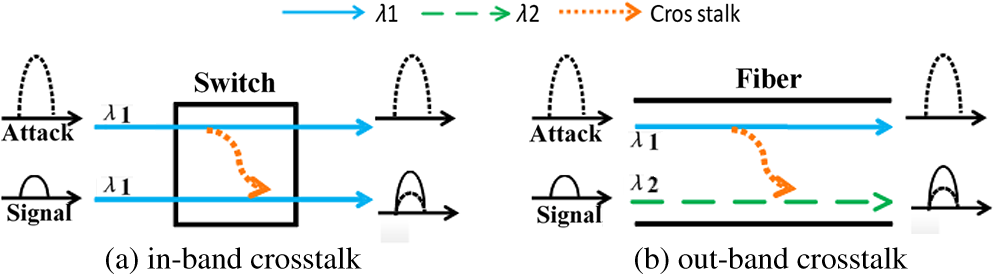
\includegraphics[scale= 0.6]{img/attackware.png}
	\caption{{\em Attack Aware Inband and Out-of-band}}
	%	\label{triangleQG}
\end{figure}



Optical Amplifiers (QA), are normally used to amplify the signal that is attenuated during the transmission process. One of the characteristics of an optical amplifier in the network is gain competition. It is necessary that the signal remains in the optical domain while traversing through the optical fiber, the signal needs proper gain in order maintain the QoS. Erbium-doped Fiber Amplifiers are(EDFAs), are commonly used operating at a wavelength region of 1550 nm, with the approximate gain of 35 nm.

\begin{figure}[h!]
	\centering
	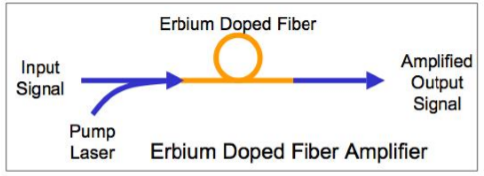
\includegraphics[scale= 0.9]{img/amplifier.png}
	\caption{{\em Optical Amplifier(OA)}}
	%	\label{triangleQG}
\end{figure}


Suppose, the attacker injects a high-powered signal at carrier wavelength λ1 (which is usually varies from 20dB to 30 dB larger than the ideal user signal) into a transparent optical network.


While traversing through the amplifier, as the amplifier can not distinguish between the attack signal and the legitimate network signals, attack signal can acquire more energy and additionally amplify its power. As a result, channel λ1 interfere with channel λ2 of power and further propagates down the network stream through the successive optical components, affecting other adjacent channels in the optical network along with propagation route and causing degrading or denying network service.


\begin{figure}[h!]
	\centering
	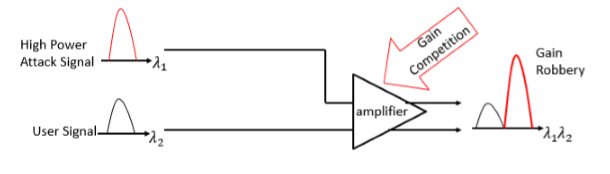
\includegraphics[scale= 0.9]{img/amplifierattack.png}
	\caption{{\em Gain Competition in amplifiers}}
	%	\label{triangleQG}
\end{figure}

\section{Attack Management Techniques}

To overcome  the effects of attacks and faults in optical networks,  two main strategies are used: protection and restoration strategies. In protection based approaches, the backup resources are reserved in advance in case of any fault/attack, while in restoration based approaches, spare backup resources are detected after diagnosing the failure in the network.


Protection techniques are further divided into link protection or path protection. In case of link protection, the backup paths and wavelengths are reserved for each link of primary path. These reserved resources are used by all the lightpaths traversing from the failure site including links, nodes etc or an attack. In the case of the path protection scheme, a parallel path (backup lightpath) is reserved for each primary lightpath in the network,  and is used if the primary path is affected by a failure.

Attack-Aware RWA consists of two approaches. The first approach attempts to design the network topology and route the lightpaths in a manner where they do not attack each other simultaneously. The second approach is based on path protection which is further classified into two types:


\begin{itemize}
	\item $Shared\ Path\ Protection (SPP)$
	\item $Dedicated\ Path\ Protection (DPP)$
\end{itemize}

\begin{enumerate}
	\item \textbf{Shared Path Protection (SPP):} In this approach, concept behind this protection scheme is to share a backup channel among different, link/node diverse, primary paths. In other words, one backup channel can be used to protect various primary paths as shown on the figure below where the link between 1 and 3 is used to protect both {\em blue} and {\em purple} color primaries. if corresponding primary paths are link-disjoint.
	\begin{figure}[h!]
		\centering
		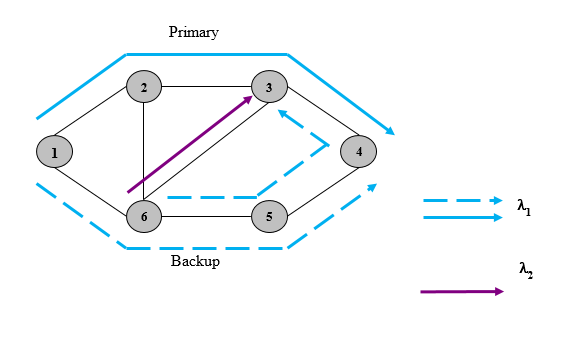
\includegraphics[scale= 1.0]{img/sharedpath.png}
		\caption{{\em Shared Path Protection}}
		%	\label{triangleQG}
	\end{figure}
	\item \textbf{Dedicated Path Protection (DPP):} In this approach, a separate backup lightpath is assigned for each primary lightpath in the optical network. If the working or primary lightpath is being attacked by a high-powered signal at a certain node or a certain link then the data transmitted over that path will be interrupted, then the data will not reach its destination rightfully. Therefore, a parallel lightpath (backup lightpath) is required that does not share resources (like nodes or links) with the primary lightpath to isolate that attacked part of the primary lightpath. The backup lightpath is utilized only if there is an attack on the primary lightpath. DPP is easier to implement and test as well as it is faster in the recovery process. For these reasons, this is the protection scheme we are going to use in our research.
	
	\begin{figure}[h!]
		\centering
		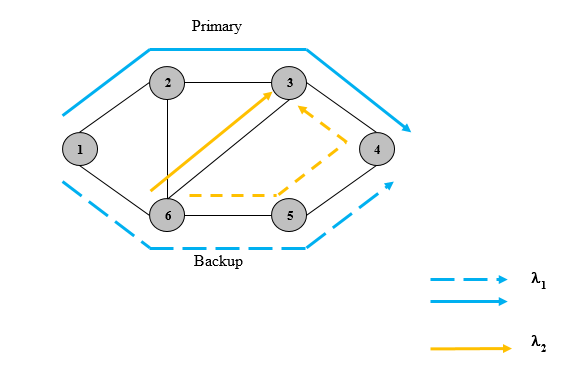
\includegraphics[scale= 1.0]{img/dedicatedpath.png}
		\caption{{\em Shared Path Protection}}
		%	\label{triangleQG}
	\end{figure}

In the figure [2.12] dedicated path protection primary and backup lightpath should be edge-disjoint in the figure above distinct color are used for different wavelengths, solid blue color and solid yellow line represents the primary lightpath where as dotted line represents backup lightpaths.  If the working or primary lightpath is being attacked by a high-powered signal at a certain node or a certain link then the data transmitted over that path will be interrupted. Then the backup lightpath will be used to accommodate the request that does not share resources.
\end{enumerate}


\section{Literature Review}


This section discusses relevant research for handling in-band and out-of-band jamming attacks in optical fiber networks. These papers propose a broad range of solution approaches, and are tested under different traffic topology, demand set and attack scenarios.


In \cite{skorin2010new}, the authors proposed the idea of routing the lightpaths in a network to reduce the damage of an attack with additional cost. The authors proposed an ILP to solve the problem for small networks to handle the out-of-band and in-band attacks. For large networks they proposed a tabu search algorithm for attack-aware lightpath routing, in combination with an existing graph-coloring algorithm for wavelength assignment. The main objective of the this ILP is to minimize the Maximum link-share attack radius (maxLAR). The secondary objective of this formulation is to reduce the average load on the network.


The authors in \cite{el2015attack} proposed a heuristic and added a new objective criterion for the RWA problem to handle in-band attack propagation in all optical WDM networks using dynamic demands traffic model. In this problem they have considered both in-band and out-of-band attack propagation. They are considering interference on first and second adjacent channels. They also consider the RWA problem with DPP.


In \cite{furdek2016attack}, the authors address the problem of routing and wavelength assignment survivability. In this paper, the authors use the concept of Attack Group(AG) of each lightpath and specify an exclusive backup path for each lightpath, which cannot be attacked by the same attacker signal. The authors use the concept of the Attack Groups to enhance the existing survivability approaches. This concept is utilized in combination with dedicated path protection(DPP) to develop an attack aware DPP(AA-DPP). A two-step approach is proposed, which solves the routing and the WA phases separately. The objective of the routing phase of AA-DPP-ILP, is to minimize the number of attack-unprotected connections under the assumption that an attack inserted on a working path can degrade any other working or backup path if they share a common link. A heuristic is used to solve routing and wavelength assignment problem for primary and backup paths. The author claims that numerical results indicate that the proposed approaches provide dedicated path protection schemes with enhanced attack protection without using more resources (i.e., wavelengths, average path lengths) than standard DPP methods.


In \cite{furdek2013attack} the authors, discuss the problem of routing and wavelength assignment survivability. They combine the conventional survivability approach with the previously proposed attack aware RWA to organise lightpaths in a way that reduces the potential damage from attacks \cite{skorin2010new} \cite{furdek2011compound}. The goal is to make the protection paths valid for attacks and not just link failures. The main focus of the work is implementing the attack aware dedicated path protection scheme, considering that the backup paths are calculated and reserved at lightpath setup time and resources may not be shared among backup paths of different connections. The attack survivable RWA algorithm is concerned about reducing the maximum potential damage from jamming attacks by minimizing the objective wavelength usage the Attack Radius (AR), as well as minimizing wavelength usage.


In \cite{furdek2014shared}, the authors state that conventional network survivability approaches protect transmission in case of the failures but do not provide good protection from the in-band or out-of-band jamming signal in the static environment since the primary and backup paths can be under the influence of same attack signal. The authors introduce a new protection scheme for jamming aware shared path protection (JA-SPP) to achieve better survivability in the presence of attack signals in a resourceful manner.  In this paper, JA-SPP claims to protect against both single link failures as well as high power jamming, with the same resource usage efficiency as standard single link failure SPP with no jamming-awareness.



\begingroup
\scriptsize

\begin{center}
	
	
	\begin{tabular}[!htbp] {|m{0.8cm}|m{2.2cm}|m{2.5cm}|m{1.5cm}|m{2.0cm}|m{2.75cm}|}
		\hline
		  \textbf{R.No.} &	\textbf{Reference} &	\textbf{Types of attacks} &	\textbf{Traffic Model}&	\textbf{Protection Scheme} &	\textbf{Solution Approach} \\ \hline
		\cite{skorin2010new}&	SkorinKapov,N., et al.2010 & 	Out-of-band and Gain competition attacks &	Static &	No &	ILP/Heuristic \\ \hline
		\cite{el2015attack} &	Marcel El Soury et al. 2015  &	Out-of-band and In-band Attacks &	Dynamic	& DPP &	Heuristic \\ \hline
		\cite{furdek2016attack} &	 Lena Wosinska et al.2016 &	In-band Attack &	Static &	DPP	& ILP/Heuristic \\ \hline
		\cite{furdek2013attack} &	Marija Furdek et al.2013 &	In-band and Out-of-band Attacks &	Static & 	DPP &	Heurstic \\ \hline
		\cite{furdek2016attack}&	Nina Skorin-Kapov et al.2014 &	In-band and Out-of-band Attacks &	Static &	SPP &	ILP \\ \hline
		
	\end{tabular}
	\captionof{table}{Summarizes all the papers we discussed under the current section. }
\end{center}

\endgroup

\chapter{Proposed Formulation For Attack-Aware RWA}

In this chapter, we are going to discuss our proposed approach for solving the attack aware routing and wavelength assignment for dynamic traffic model, using dedicated path protection. This chapter includes the detailed illustration and presentation of the ILP formulation (including objectives, set of constraints) and other key features of the solution. The main objective of the ILP formulation is to maximize the number of successful requests in the network, while minimizing the path lengths of all the primary and backup paths.


\section{Synopsis Of Proposed Model}

In our proposed model, the physical topology of the network is represented by a directed graph $Gp = (Vp, Ep)$, where $Vp$ is the set of nodes and $Ep$ is the set of edges. In this network each link is considered as bi-directional, which is implemented by a pair of uni-directional links in the physical topology. Figure [3.1] shows an example of a network topology with 6 nodes and 8 physical links (bi-directional).



\begin{figure}[h!]
	\centering
	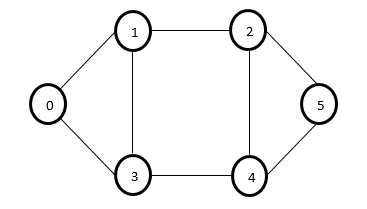
\includegraphics[scale= 1.0]{img/6node.png}
	\caption{{\em 6-node physical network topology}}
	%	\label{triangleQG}
\end{figure}

There are multiple ways to handle the malicious spread of the high-powered jamming signal in TON’s. Major part of the research, considering attacks handling approaches are reactive in nature as they concentrate more on the network recovery \cite{furdek2011physical} after experiencing an attack. In this thesis, the attack handling procedures are incorporated within the planning phase \cite{furdek2011physical}. The thesis also takes into consideration the fact that the interference and crosstalk between the channels sharing same link decreases as the channel spacing between their assigned channels increases \cite{tripathi2007reduction}. Hence, the actual value of the channel spacing for which the crosstalk may be ignored depends upon the number of factors such as the signal strength of the attacking and attacked signal, the type of modulation used for sending out the signal onto the fiber and the properties of the fiber \cite{zhao2016attack}.


Figure [3.2] shows a fiber with 5 available channels, numbered 1 to 5. If an attacking signal is introduced on channel 3. It will attack lightpaths on adjacent channels only (i.e. channel 2 and channel 4). However, signals on channels 1 and 5 will not be affected by this attack. We are considering this model approach in our thesis and neglecting the second adjacent channels, as discussed in the previous work the inference or leaking of the attacking signal to the second adjacent channel is almost zero.

\begin{figure}[h!]
	\centering
	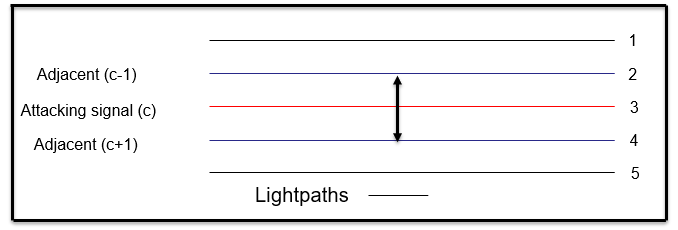
\includegraphics[scale= 0.8]{img/attack_fibers.png}
	\caption{{\em Considering first adjacent channel}}
	%	\label{triangleQG}
\end{figure}


\section{Proposed ILP Formulation For Dynamic Attack-Aware RWA (DAA-RWA)}

In this section, we present the ILP formulation for the attack aware RWA for the dynamic traffic model. Different constraints are proposed in order to reduce the disruption in the network by malicious attacks (in-band and out-of-band attacks) for the new and existing primary and backup lightpaths.

\subsection{Notation:}

The following notation are used in the proposed ILP formulation.

\subsection{Input parameters:}

\begin{itemize}
	\item 	A physical topology $G [N, A]$.
	\item	N : Set of nodes.
	\item	A : The set of all edges (physical fiber links) between the nodes of the network.
	\item	C : Set of channel numbers.
	\item	K : Set of all on-going communication.
	\item	M : A large constant.
	\item	$a_{i,j}^{c,k}$ : A constant for channel $c \in C$ on edge $(i,j) \in A $ and primary lightpath $k$ such that $1$ if channel $c$ on edge $(i,j) \in A $ is used by the $k^{th}$ primary lightpath, $0$ otherwise.
	\item	$p_i^{c,k}$ : A constant for channel  $c \in C$, node $i \in N $ and primary lightpath $k$ such that $1$ if the $k^{th}$ primary lightpath uses node $i \in N $ and channel $c$, $0$ otherwise.
	\item	$b_{i,j}^{c,k}$ : A constant for channel $c \in C$ on edge $(i,j) \in A $ and communication $k$ such that $1$ if channel $c$ on edge $(i,j) \in A $ is used by the $k^{th}$ backup lightpath, $0$ otherwise.
	\item	$q_i^{c,k}$ : A constant for channel $c \in C$, node $i \in N $ and backup lightpath $k$ such that $1$ if the kth backup lightpath uses node $i \in N $ and channel $c$, $0$ otherwise.
	\item	S : Source node of request.
	\item	D : Destination node of request.
	
\end{itemize}

\subsection{Variables:}

\begin{itemize}
	\item 	$x_{i,j}$  : A binary variable denoting whether the path chosen for the primary lightpath uses edge $(i,j) \in A $,  where $x_{i,j}$ = 1, if the path chosen for the primary lightpath uses edge $(i,j) \in A $, 0 otherwise.
	\item 	$y_{i,j}$  : A binary variable denoting whether the path chosen for the backup lightpath uses edge $(i,j) \in A $, where $y_{i,j}$ = 1, if the path chosen for the backup lightpath uses edge $(i,j) \in A $, 0 otherwise.
	\item 	$\omega^c$ : A binary variable denoting the channel used for the primary lightpath such that $\omega^c$ = 1, if the primary lightpath for the new connection request uses channel $c$, 0 otherwise.
	\item 	$\nu^c$ : A binary variable denoting the channel used for the primary lightpath such that $\nu^c$ = 1, if the backup lightpath for the new connection request uses channel $c$, 0 otherwise.
	\item 	$\gamma_{i,j}^c$ : A continuous variable where the value lies between 0 and 1, $\gamma_{i,j}^c$ = 1, if the new primary lightpath uses channel $c$ and edge $(i,j) \in A $, 0 otherwise.
	\item 	$\delta_{i,j}^c$ : A continuous variable where the value lies between 0 and 1, $\delta_{i,j}^c$ = 1, if the new backup lightpath uses channel $c$ and edge $(i,j) \in A $, 0 otherwise.
	\item 	$R1^k$ : A binary variable where $R1^k$ = 1, if the new primary lightpath may attack the $k^{th}$ primary lightpath, 0 otherwise.
	\item 	$S1^k$ : A binary variable where $S1^k$ = 1, if the new primary lightpath may attack the $k^{th}$ backup lightpath, 0 otherwise.
	\item 	$R2^k$ : A binary variable where $R2^k$ = 1, if the new backup lightpath may attack the $k^{th}$ primary lightpath, 0 otherwise.
	\item   $S2^k$ : A binary variable where $S2^k$ = 1, if the new backup lightpath may attack the $k^{th}$ backup lightpath, 0 otherwise.
	\item   $s$ : A binary variable where $s$ = 1, if the request for a connection may be satisfied, 0 otherwise.
	
\end{itemize}


\section{ILP Formulation (DAA-RWA)}

\subsection{Objective function}

Maximize $$M \cdot s - \sum_{(i,j)\in A} x_{ij} - \sum_{(i,j)\in A} y_{ij}$$


Satisfy the flow-balance equations for the primary and the backup lightpaths:


\begin{equation}
\label{eq1}
\sum_{j:(i\rightarrow j)\in A} x_{ij} - \sum_{j:(j\rightarrow i)\in A} x_{ji} = \left\{
\begin{array}{l l l}
s & \mbox{if $i = S$ }\\
-s &  \mbox{if $i = D$}  , \emph{i} \in \emph{N},\\
0 &  \mbox{otherwise.}
\end{array} \right.
\end{equation}

\begin{equation}
\label{eq2}
\sum_{j:(i\rightarrow j)\in A} y_{ij} - \sum_{j:(j\rightarrow i)\in A} y_{ji} = \left\{
\begin{array}{l l l}
s & \mbox{if $i = S$ }\\
-s &  \mbox{if $i = D$}  , \emph{i} \in \emph{N},\\
0 &  \mbox{otherwise.}
\end{array} \right.
\end{equation}

Primary and backup paths must be edge disjoint

\begin{equation}
\tag{3}\label{eq3}
x_{i,j} + y_{i,j} \leq 1 \quad \forall (i,j) \in A
\end{equation}

Wavelength continuity constraints

\begin{equation}
\tag{4a}\label{eq4a}
\sum_{c\in C} \omega^c = s  \quad  \forall c \in \mathcal{C}
\end{equation}

\begin{equation}
\tag{4b}\label{eq4b}
\sum_{c\in C} \nu^c = s  \quad \forall c \in \mathcal{C}
\end{equation}

\begin{equation}
\tag{4c}\label{eq4c}
\omega^c+\nu^c \leq 1  \quad \forall c \in \mathcal{C}
\end{equation}


Define $\gamma_{i,j}^c$ and $\delta_{i,j}^c$


\begin{equation}
\tag{5a}\label{eq5a}
\Upsilon^{c}_{ij} \leq \omega^c  \quad \forall (i,j) \in A, \forall c \in \mathcal{C}
\end{equation}



\begin{equation}
\tag{5b}\label{eq5b}
\Upsilon^{c}_{ij} \leq x_{ij}  \quad \forall (i,j) \in A, \forall c \in \mathcal{C}
\end{equation}

\begin{equation}
\tag{5c}\label{eq5c}
\Upsilon^{c}_{ij} \geq \omega^c + x_{ij} - 1  \quad \forall (i,j) \in A, \forall c \in \mathcal{C}
\end{equation}


\begin{equation}
\tag{6a}\label{eq6a}
\delta^{c}_{ij} \leq \nu^c  \quad \forall (i,j) \in A, \forall c \in \mathcal{C}
\end{equation}

\begin{equation}
\tag{6b}\label{eq6b}
\delta^{c}_{ij} \leq y_{ij}  \quad \forall (i,j) \in A, \forall c \in \mathcal{C}
\end{equation}

\begin{equation}
\tag{6c}\label{eq6c}
\delta^{c}_{ij} \geq \nu^c + y_{ij} - 1  \quad \forall (i,j) \in A, \forall c \in \mathcal{C}
\end{equation}

Wavelength clash constraints


\begin{equation}
\tag{7a}\label{eq7a}
\Upsilon^c_{ij}  + \sum_{k\in K} a^{ck}_{ij} + \sum_{k\in K} b^{ck}_{ij} \leq 1 \quad \forall (i,j) \in A, \forall c \in \mathcal{C}
\end{equation}


\begin{equation}
\tag{7b}\label{eq7b}
\delta^c_{ij}  + \sum_{k\in K} a^{ck}_{ij} + \sum_{k\in K} b^{ck}_{ij} \leq 1 \quad \forall (i,j) \in A, \forall c \in \mathcal{C}
\end{equation}


Set  $R1^k$ = 1, if new primary lightpath may attack $k^{th}$ existing primary lightpath


\begin{equation}
\tag{8a}\label{eq8a}
R1^k \geq \Upsilon^{c}_{ij} \cdot  p^{ck}_{i}  \quad \forall (i,j) \in A, \forall k \in K, \forall c \in \mathcal{C}
\end{equation}

\begin{equation}
\tag{8b}\label{eq8b}
R1^k \geq \Upsilon^{c}_{iD} \cdot  p^{ck}_{D}  \quad \forall (i,j) \in A, \forall k \in K, \forall c \in \mathcal{C}
\end{equation}

\begin{equation}
\tag{8c}\label{eq8c}
R1^k \geq \Upsilon^{c}_{ij} \cdot (a^{(c-1)k}_{ij} + a^{(c+1)k}_{ij})  \quad \forall (i,j) \in A, \forall k \in K, \forall c \in \mathcal{C}
\end{equation}

\begin{equation}
\tag{8d}\label{eq8d}
R1^k \leq \sum_{(i, j) \in A} \sum_{c \in \mathcal{C}} \Upsilon^{c}_{ij} \cdot [(a^{(c-1)k}_{ij} + a^{(c+1)k}_{ij}) +  p^{ck}_{i} + p^{ck}_{D}] \quad  \forall k \in K
\end{equation}


Set  $S1^k$ = 1, if new primary lightpath may attack $k^{th}$ existing backup lightpath


\begin{equation}
\tag{9a}\label{eq9a}
S1^k \geq \Upsilon^{c}_{ij} \cdot  q^{ck}_{i}  \quad \forall (i,j) \in A, \forall k \in K, \forall c \in \mathcal{C}
\end{equation}

\begin{equation}
\tag{9b}\label{eq9b}
S1^k \geq \Upsilon^c_{iD} \cdot  q^{ck}_{D}  \quad \forall k \in K, \forall c \in \mathcal{C}
\end{equation}

\begin{equation}
\tag{9c}\label{eq9c}
S1^k \geq \Upsilon^{c}_{ij} \cdot (b^{(c-1)k}_{ij} + b^{(c+1)k}_{ij})  \quad \forall (i,j) \in A, \forall k \in K, \forall c \in \mathcal{C}
\end{equation}

\begin{equation}
\tag{9d}\label{eq9d}
S1^k \leq \sum_{(i, j) \in A} \sum_{c \in \mathcal{C}} \Upsilon^{c}_{ij} \cdot [(b^{(c-1)k}_{ij} + b^{(c+1)k}_{ij}) +  q^{ck}_{i} + q^{ck}_{D}] \quad  \forall k \in K
\end{equation}



Set  $R2^k$ = 1, if new backup lightpath may attack $k^{th}$ existing primary lightpath


\begin{equation}
\tag{10a}\label{eq10a}
R2^k \geq \delta^{c}_{ij} \cdot  p^{ck}_{i}  \quad \forall (i,j) \in A, \forall k \in K, \forall c \in \mathcal{C}
\end{equation}

\begin{equation}
\tag{10b}\label{eq10b}
R2^k \geq \delta^{c}_{iD} \cdot  p^{ck}_{D}  \quad \forall (i,j) \in A, \forall k \in K, \forall c \in \mathcal{C}
\end{equation}

\begin{equation}
\tag{10c}\label{eq10c}
R2^k \geq \delta^{c}_{ij} \cdot (a^{(c-1)k}_{ij} + a^{(c+1)k}_{ij})  \quad \forall (i,j) \in A, \forall k \in K, \forall c \in \mathcal{C}
\end{equation}

\begin{equation}
\tag{10d}\label{eq10d}
R2^k \leq \sum_{(i, j) \in A} \sum_{c \in \mathcal{C}} \delta^{c}_{ij} \cdot [(a^{(c-1)k}_{ij} + a^{(c+1)k}_{ij}) +  p^{ck}_{i} + p^{ck}_{D}] \quad  \forall k \in K
\end{equation}


Set  $S2^k$ = 1, if new backup lightpath may attack $k^{th}$ existing backup lightpath



\begin{equation}
\tag{11a}\label{eq11a}
S2^k \geq \delta^{c}_{ij} \cdot  q^{ck}_{i}  \quad \forall (i,j) \in A, \forall k \in K, \forall c \in \mathcal{C}
\end{equation}

\begin{equation}
\tag{11b}\label{eq11b}
S2^k \geq \delta^c_{iD} \cdot  q^{ck}_{D}  \quad \forall k \in K, \forall c \in \mathcal{C}
\end{equation}

\begin{equation}
\tag{11c}\label{eq11c}
S2^k \geq \delta^{c}_{ij} \cdot (b^{(c-1)k}_{ij} + b^{(c+1)k}_{ij})  \quad \forall (i,j) \in A, \forall k \in K, \forall c \in \mathcal{C}
\end{equation}

\begin{equation}
\tag{11d}\label{eq11d}
S2^k \leq \sum_{(i, j) \in A} \sum_{c \in \mathcal{C}} \delta^{c}_{ij} \cdot [(b^{(c-1)k}_{ij} + b^{(c+1)k}_{ij}) +  q^{ck}_{i} + q^{ck}_{D}] \quad  \forall k \in K
\end{equation}



If the new primary lightpath attacks any existing primary lightpaths, it must not attack the corresponding existing backup lightpaths.


\begin{equation}
\tag{12}\label{eq12}
R1^k + S1^k \leq 1 \quad \forall k \in K
\end{equation}


If the new backup lightpath attacks any existing primary lightpaths, it must not attack the corresponding existing backup lightpaths.


\begin{equation}
\tag{13}\label{eq13}
R2^k + S2^k \leq 1 \quad \forall k \in K
\end{equation}



If the $k^{th}$ existing primary lightpath attacks the new primary lightpaths, it must not attack the corresponding new backup lightpath.

\begin{equation}
\tag{14}\label{eq14}
R1^k + R2^k \leq 1 \quad \forall k \in K
\end{equation}

If the $k^{th}$ existing backup lightpath attacks the new primary lightpaths, it must not attack the corresponding new backup lightpath.

\begin{equation}
\tag{15}\label{eq15}
S1^k + S2^k \leq 1 \quad \forall k \in K
\end{equation}








\section{Justification of ILP Constraints}


The objective function of the ILP formulation is to maximize the number of requests that can be established in the network, by carrying out dynamic attack-aware RWA for each request. In our objective we used {\em M} which is a large constant multiplied with {\em s} request satisfying binary variable, the value will be 1, if the corresponding request for a connection is satisfied, otherwise the value will be 0. The constraints {\em (1)-(2)} are the flow balance, basic routing and wavelength assignment constraints for primary and backup lighpaths. The constraints  {\em (1-2)} are the traditional flow conservation constraints that allocate a feasible route  to the lightpath over the physical topology. The constraint {\em (3)} is the edge disjoint constraint, ensuring that the new primary lightpath and the new backup lightpath do not have any common edges. The constraint {\em (4a)-(4c)} enforces the wavelength continuity constraint for the new primary (backup) lightpath. This ensures that the same wavelength $c$ is allotted to the lightpath  throughout its route. The constraints {\em (5a)-(5c)}  compute the continuous variable $ \gamma_{i,j}^c $ such that $ \gamma_{i,j}^c = 1$ if the new primary lightpath uses channel $c$ and edges $ (i, j) \in A$. Similarly, the constraints {\em (6a)-(6c)}  compute the continuous variable $ \delta_{i,j}^c $ such that $ \delta_{i,j}^c = 1$ if the new backup lightpath uses channel $c$ and edges $(i, j) \in A $. The constraints {\em (7a)-(7b)} are wavelength clash constraints. The constraint {\em (7a)-(7b)} states that a channel $c$ on edge $(i, j) \in A $ can be used by the primary (backup) lightpath of the new request only if it is not currently allocated to any existing primary or backup lightpath.


The constraints {\em (8a)-(8d)} are attack aware constraints. The constraints {\em (8a)-(8d)} set the value of $R1^k = 1$ if the new primary lightpath is capable of attacking the $k^{th}$ existing primary lightpath and vice versa. The constraints {\em (8a)-(8b)} are used to address the case of in-band attacks, and set $R1^k = 1$ if the new primary lightpath and the $k^{th}$ existing primary lightpath both use the same wavelength $c$ and share a common node $i$.  The constraint {\em (8c)} is for out-of-band attack in the network and sets the value of $R1^k = 1$ if the new primary lightpath and $k^{th}$ primary lightpath share a common link $(i,j)$ and the channels allocated to these two lightpaths are adjacent to each other. In other works, if the new primary lightpath uses channel $c$ (i.e. $\omega_c = 1$ and the $k^{th}$ primary lightpath uses channel $c+1$ or $c-1$. Finally, constraint {\em(8d)} ensures that the value of $R1^k$ is set to 0 if none of the conditions of in-band and out-of-band attacks are between the new primary lightpath and $k^{th}$ existing primary lightpath are not satisfied, i.e. they are not able to attack each other.


Constraints {\em (9a)-(9d)} are similar to constraints {\em (8a)-(8d)}, but are used to determine if the new primary lightpath is capable of attacking the $k^{th}$ existing \emph{backup} lightpath and vice versa. If so, the value of $S1^k$ is set to 1, and 0 otherwise. In a similar manner, constraints {\em (10a)-(10d) ((11a) - (11d))},  are used to determine if the new backup lightpath is capable of attacking the $k^{th}$ existing primary (backup) lightpath and vice versa. If so, the value of $R2^k$ ($S2^k$) is set to 1, and 0 otherwise.

The constraint {\em (12)} ensures that it is not possible for the new primary lightpath to attack both the $k^{th}$ existing primary and backup lightpaths at the same time (i.e., the $k^{th}$ existing primary and backup lightpaths are not within the reach of the same attacker).

The constraint {\em (13)} ensures that it is not possible for the new backup lightpath to attack both the $k^{th}$ existing primary and backup lightpaths at the same time (i.e., the $k^{th}$ existing primary and backup lightpaths are not within the reach of the same attacker).

The constraint {\em (14)} ensures that it is not possible for the $k^{th}$  primary lightpath to attack both the new primary and backup lightpaths at the same time.  Finally, constraint {\em (15)} ensures that it is not possible for the $k^{th}$  bakcup lightpath to attack both the new primary and backup lightpaths at the same time.


\section{An Illustrative Example}

An illustrative example is discussed in this section in order to explain the proposed approach. While using the DPP approach, two lightpaths must be established in order to support each connection request between a pair of source and destination nodes. The first is the primary path or working path and the other is known as backup lightpath. The backup lightpath is not used unless the primary lightpath is disrupted, either due to a fault in the network or an attack.

Figure 3.3 shows 2 connections established over a 6-node physical topology. $r1_w$ and $r1_b$ ($r2_w$ and $r2_b$) are the primary and backup lightpaths of the first (second) connection respectively.  $r1_w$ and $r1_b$ use routes $0 \rightarrow 2 \rightarrow 5$ and $0 \rightarrow 1 \rightarrow 4 \rightarrow 5$ and are assigned channels $\lambda_1$ and $\lambda_2$ respectively. $r2_w$ and $r2_b$ use routes $1 \rightarrow 4 $ and $1 \rightarrow 0 \rightarrow 2 \rightarrow 5 \rightarrow 4$ and are  assigned channels $\lambda_3$ and $\lambda_2$ respectively.

This means that $r2_b$ can attack $r1_w$ using out-of-band attack, since they are assigned adjacent channels on a common link $2 \rightarrow 5$. Moreover,  $ r2_b $, it can also attack (using in-band attack) lightpath $r1_b$, as they are using a common channel $\lambda_2$ and traversing the same nodes (at nodes 0, 1, 4 and 5). This violates constraint \emph{(13) } and therefore is not a valid attack-aware RWA.



\begin{figure}[h!]
	\centering
	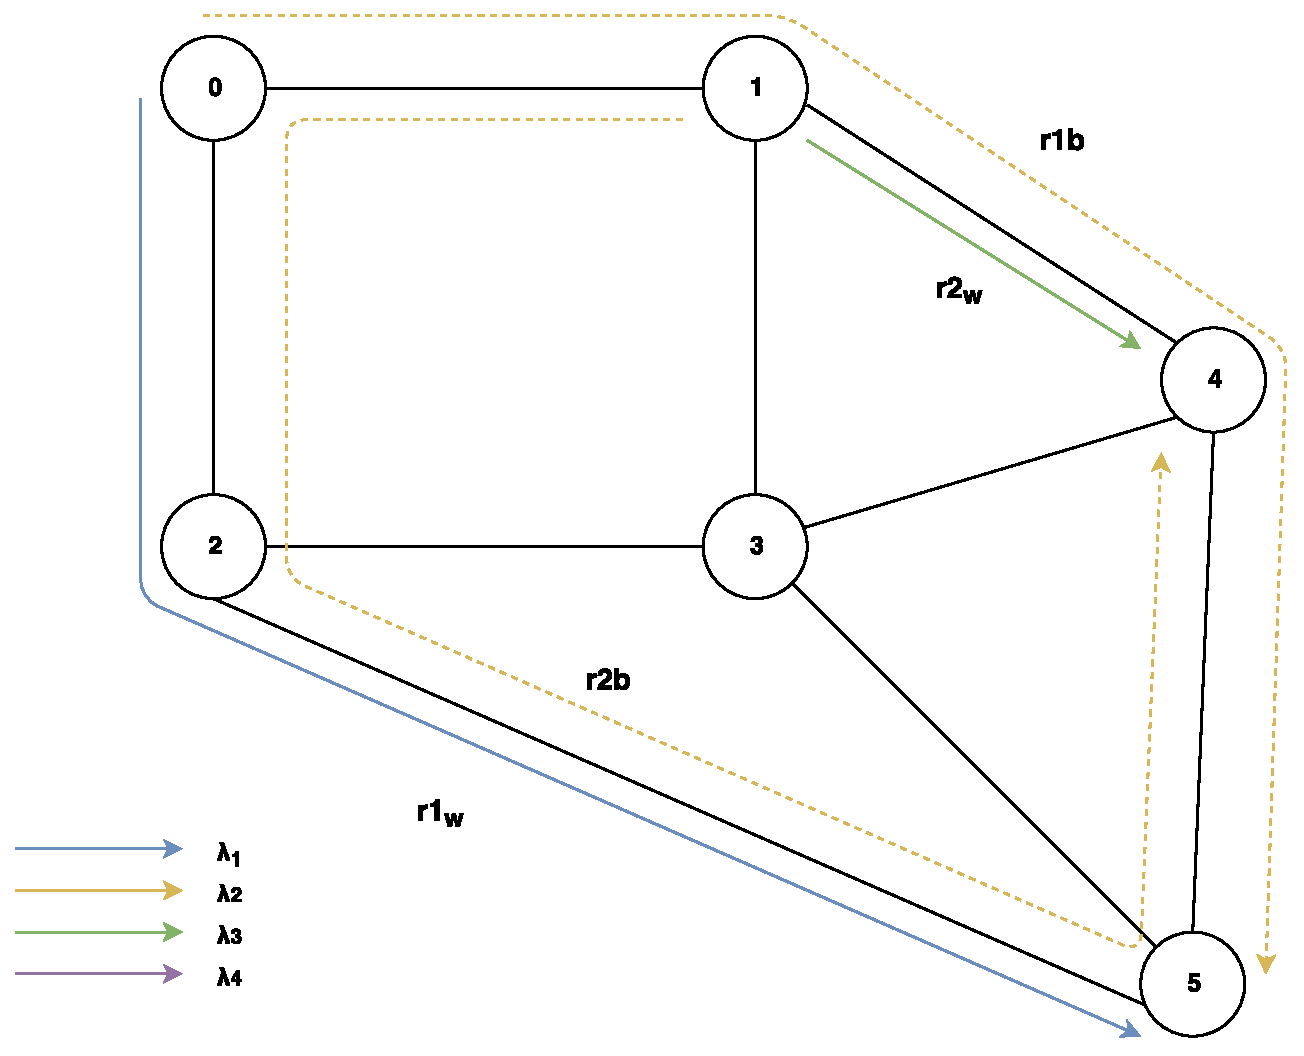
\includegraphics[scale= 0.6]{img/attackwarepdf.pdf}
	\caption{{\em Illustration of invalid Attack-aware RWA}}
	%	\label{triangleQG}
\end{figure}

On the other hand, if we assign wavelength $\lambda_4$ for lightpath $r1_w$ then, $r2_b$ can no longer attack $r1_w$, since the two lightpaths are no longer using adjacent channels. This would be a valid attack- aware RWA, and is shown below in Figure 3.4.

\begin{figure}[h!]
	\centering
	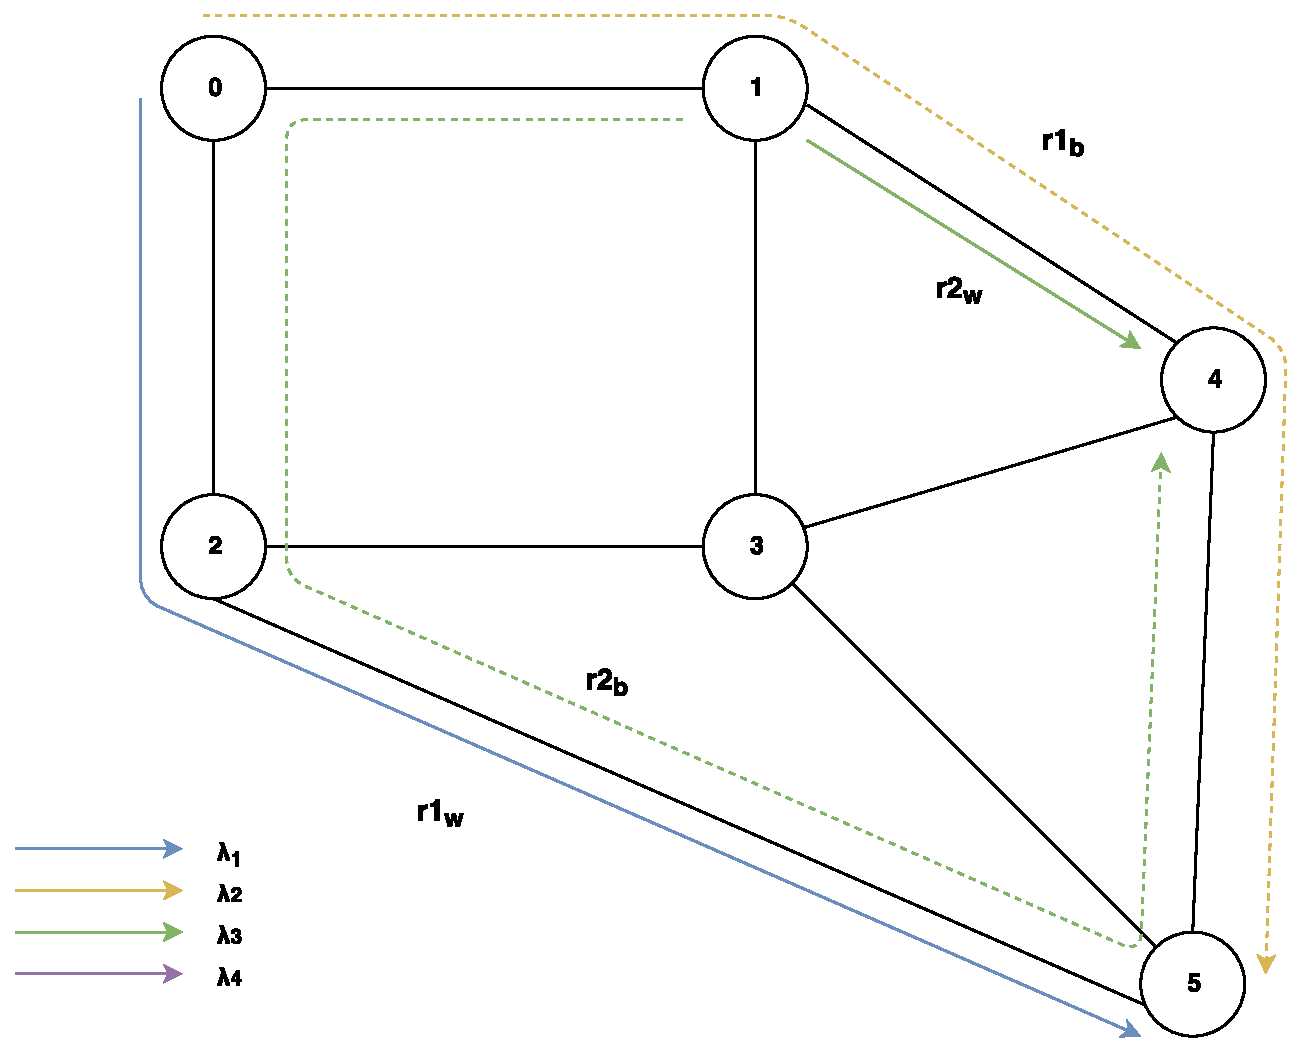
\includegraphics[scale= 0.6]{img/validAttackaware.pdf}
	\caption{{\em Illustration of valid Attack-aware RWA}}
	%	\label{triangleQG}
\end{figure}

\chapter{Experiments And Results}

In this chapter we present our simulations and discuss the results for different network topologies. We compare the performance of our proposed approach (DAA-RWA), outlined in Chapter 3, with the with the following two approaches: 
\begin{itemize}
  \item A full attack-aware RWA approach using dedicated protection (AA-DPP) \cite{furdek2013attack}
  \item An attack-unaware RWA approach that minimizes the number of wavelength links (AU-RWA)
\end{itemize}

The main objective is to minimize the blocking probabilities. The proposed ILP can generate optimal results for practical sized problems, using the IBM ILOG CPLEX 12.6.2 optimization studio \cite{nizampatnam2017minimizing}.
The {\em blocking probability} is a measure of the probability that an incoming call request will be denied. It depends on factors such as offered traffic, network resources and connection control algorithms. The blocking probability can be used as a metric for evaluation of various protection schemes. A scheme which has a lower blocking probability makes better utilization of the network resources. An increase in number of set up requests means a decrease in the lightpath blocking probability, therefore a better network performance \cite{sen2003preemptive}.


\section{Simulation Setup}


In our simulations, we experimented with the following three topologies:
\begin{enumerate}
%\item 	The 11-node COST-239 network shown in Fig 4.1 \cite{das2017dynamic},
\item	The 14-node NSFNET shown in Fig 4.2 \cite{das2017dynamic},
\item	The 20-node ARPANET network shown in Fig 4.3 \cite{das2017dynamic}
\item	A 40-node synthetic network topology
		%\begin{figure}[h!]
		%\centering
		%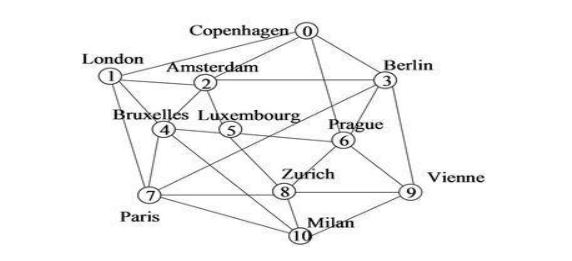
\includegraphics[scale= 1.0]{img/topology11node.png}
		%\caption{{\em COST-239 network (11 - node topology) }}
		%	\label{triangleQG}
		%\end{figure}

		\begin{figure}[h!]
		\centering
		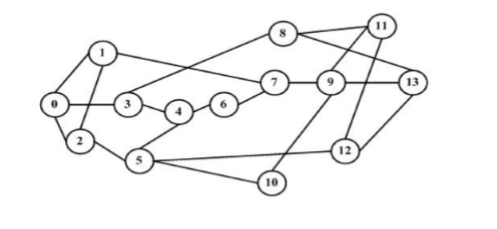
\includegraphics[scale= 1.0]{img/topology14node.png}
		\caption{{\em  NSFNET network (14 - node topology)} }
		%	\label{triangleQG}
		\end{figure}
	
		\begin{figure}[h!]
		\centering
		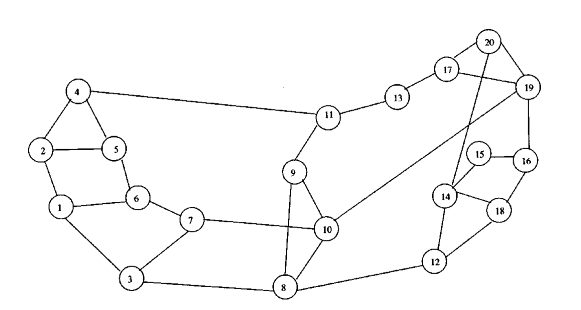
\includegraphics[scale= 1.0]{img/topology20node.png}
		\caption{{\em  ARPANET network (20 - node topology) }}
		%	\label{triangleQG}
		\end{figure}

		%\begin{figure}[h!]
		%\centering
		%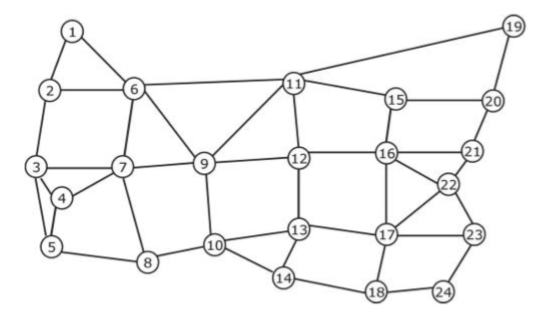
\includegraphics[scale= 1.0]{img/topology24node.png}
		%\caption{{\em  ARPANET network (24 - node topology) }}
		%	\label{triangleQG}
		%\end{figure}
\end{enumerate}

 The links between two nodes in each physical topology are assumed to be bidirectional, composed of 2 separate unidirectional optical fibers. Each fiber can support 8,16 or 32 channels. The network layout or topology is defined by the network topology file. This information is supplied in the form of a table of size $NxN$, where $N$ is the number of nodes in the network. In the table, if the value in row $i$ and column $j$ is 1(0), it means there is a link (there is no link) between node $i$ and node $j$. Figure 4.3 illustrates the structure of the topology file .


\begin{figure}[h!]
	\centering
	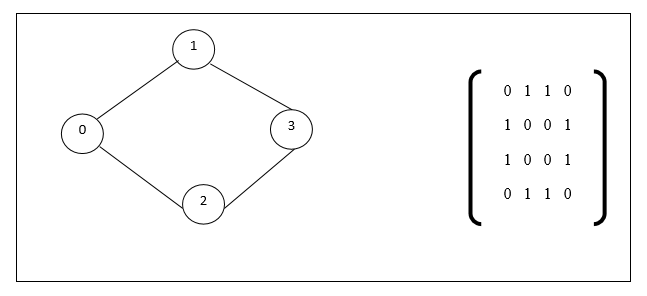
\includegraphics[scale= 0.9]{img/topologyfile.png}
	\caption{{\em Example of a 4-node network and corresponding topology file \cite{el2015attack} }}
	%	\label{triangleQG}
\end{figure}


After reading the network topology, we input the demand file. The demand file consists of a set of demands to be established over the network. Each demand consists of a source and destination node, which are randomly generated. The number of demands in a demand file ranges between 20 – 105 demands. The demands are given as input to the ILP one by one. The ILP attempts to find a feasible  primary lightpath and  backup lightpath for each demand. Two possible cases are considered:



%\begin{figure}[h!]
%	\centering
%	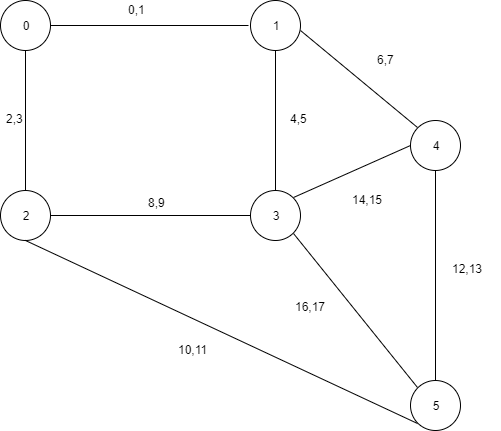
\includegraphics[scale= 0.5]{img/noofedges.png}
%	\caption{{\em Example of number the edges}}
	%	\label{triangleQG}
%\end{figure}


\begin{enumerate}
	\item	If a demand is successfully allocated, the assigned routes and channels are used to update the databases, which contain information about routes of each established connection. This information is used when trying to accommodate the next request, to ensure both primary and backup lightpaths are not simultaneously attacked by the same lightpath.
	\item	If feasible primary and backup lightpaths could not be allocated, the demand is considered ‘blocked’ and contributes to the blocking probability. In this case, there is no need to update the corresponding databases, before trying the next demand.
	
	
\end{enumerate}

\section{Blocking probability vs. Demand size}


Tables 4.1, 4.2 and 4.3 show how the blocking probability varies when the traffic load is varied for different topologies, with 16 channels per fiber. The number of demands for the first 2 networks varied from 20 - 35 demands, while for the 40-node network the number of demands varied from 90 - 105 demands. The Attack-Unaware DPP (AU-DPP) represents the traditional DPP algorithm, which does not consider potential attacks. In AU-DPP, a connection is never blocked due to vulnerability to attacking lightpaths; it can only be blocked due to unavailability of suitable channels to route the corresponding working and backup lightpaths, due to network congestion. Therefore, in all these simulations, we expect that the AU-DPP approach will have the best performance, and is included as a reference point to evaluate the other approach. As expected, the blocking probability in general increases with the requests.


\begin{table}[h!]
	\begin{center}
		\begin{tabular}{|c|c|c|c|c|} \hline
			&  \multicolumn{4}{c|}{Blocking Probability}  \\ \hline
			Traffic Load & 20 & 25 & 30 & 35	\\ \hline
			Approach & & & &   \\ \hline
			AA-DPP & 1.25 & 7 & 11.66 & 18.57 \\ \hline
			%AA-DPP(H) (i=1) & 7.25 & 7.25 & 8.66 & 15.38 \\ \hline
			%AA-DPP(H) (i=2) & 7.25 & 7.25 & 8.00 & 16.40 \\ \hline
			AU-DPP & 0 & 0 & 0 & 0 \\ \hline
			DAA-RWA & 0 & 0 & 0 & 0 \\ \hline
		\end{tabular}
	\caption{Blocking Probability vs. Demand Size - 14 nodes, 16 channels}
	\end{center}
\end{table}

For all topologies, the results indicate that the blocking probability of AA-DPP[9] approach is higher than our approach and the attack-unaware approach for all considered traffic loads. The average blocking probability of DAA-RWA is similar to AU-DPP for low traffic loads. As the traffic load increases, the difference in blocking probability between AU-DPP and the proposed approach becomes more noticeable. However, the proposed approach still consistently performs better that AA-DPP[9].



\begin{table}[h!]
	\begin{center}
		\begin{tabular}{|c|c|c|c|c|} \hline
			&  \multicolumn{4}{c|}{Blocking Probability}  \\ \hline
			Traffic Load & 20 & 25 & 30 & 35	\\ \hline
			Approach & & & &   \\ \hline
			AA-DPP & 0 & 0 & 0.83 & 2.14 \\ \hline
			%AA-DPP(H) (i=1) & 10.74 & 10.74 & 13.8 & 18.99 \\ \hline
			%AA-DPP(H) (i=2) & 10.74 & 10.74 & 13.77 & 18.69 \\ \hline
			AU-DPP & 0 & 0 & 0 & 0 \\ \hline
			DAA-RWA & 0 & 0 & 0 & 0 \\ \hline
		\end{tabular}
		\caption{Blocking Probability vs. Demand Size - 20 nodes, 16 channels}
	\end{center}
\end{table}



\begin{table}[h!]
	\begin{center}
		\begin{tabular}{|c|c|c|c|c|} \hline
			&  \multicolumn{4}{c|}{Blocking Probability}  \\ \hline
			Traffic Load & 90 & 95 & 100 & 105	\\ \hline
			Approach & & & &   \\ \hline
			AA-DPP & 58.61 &	60.52	& 61.75 &	62.85 \\ \hline
			%AA-DPP(H) (i=1) & 6.39 & 9.53 &	15.7 &	23.58 \\ \hline
			%AA-DPP(H) (i=2) & 6.22 & 8.82 &	14.67 &	21.94 \\ \hline
			AU-DPP & 25.56 &	29.47 &	33 & 36.19 \\ \hline
			DAA-RWA & 31.11	& 34.04	& 36.33 & 38.41 \\ \hline
		\end{tabular}
		\caption{Blocking Probability vs. Demand Size - 40 nodes, 16 channels}
	\end{center}
\end{table}


\begin{figure}[h!]
		\centering
		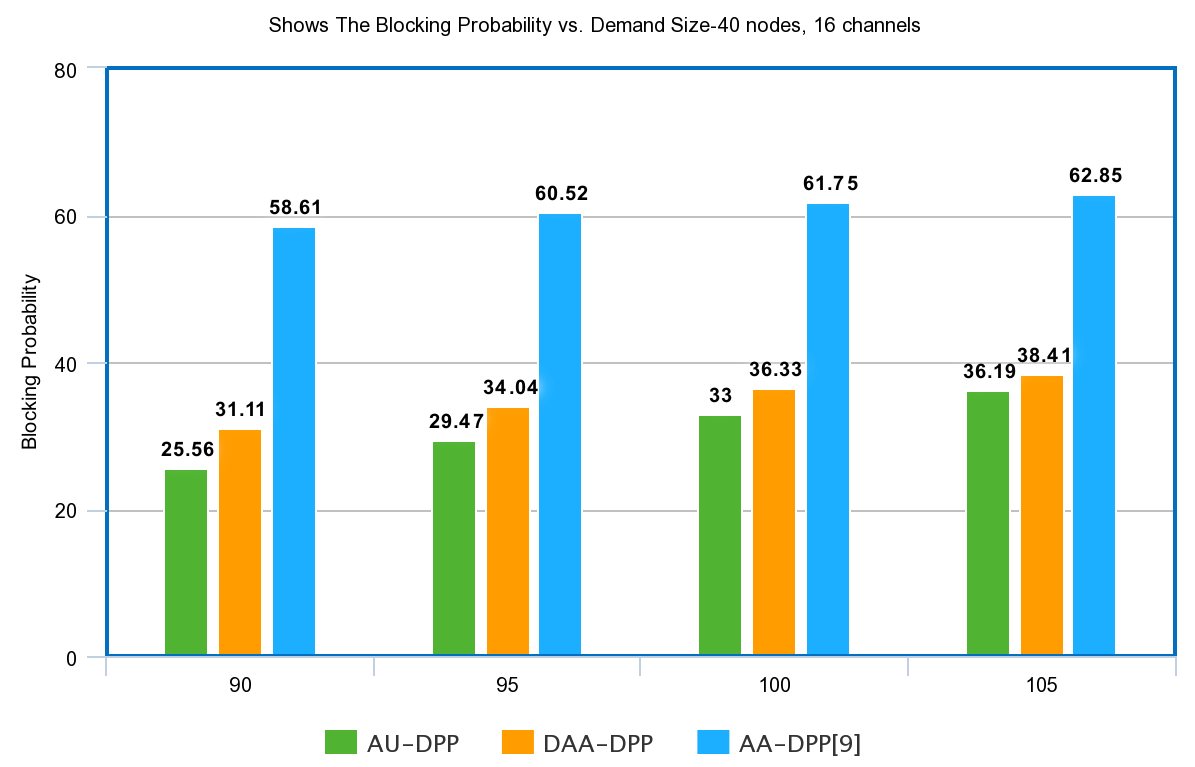
\includegraphics[scale= 0.3]{img/chart1.png}
		\caption{{\em  Comparison of blocking probabilities using different approaches }}
		%	\label{triangleQG}
		\end{figure}
		
Figure 4.5 compares the blocking probability the different approaches in the 40-node network for different traffic loads. As, expected, blocking probability of our proposed approach is more than the blocking probability of AU-DPP. However, the proposed approach still consistently performs better that AA-DPP[9].


\section{Blocking probability vs. Channels}

In this section, we study how the blocking probability varies with the number of available channels per fiber. Tables 4.4, 4.5 and 4.6 represent the blocking probability of 14-nodes, 20-nodes, and 40 nodes network using fibers with 8, 16 and 32 channels. The three tables show that the blocking probability of AA-DPP[9] consistently exceeds all the other approaches. The performance of our proposed approach is very close to that of AU-DPP, particularly when the network is less congested (i.e. more available channels per fiber). As the network congestion increases, the performance of the proposed approach degrades somewhat compared to AU-DPP, but is still better than AA-DPP. For all three approaches, the blocking probability decreases when the number of channels per fiber increases.

\begin{table}[h!]
	\begin{center}
		\begin{tabular}{|c|c|c|c|} \hline
			&  \multicolumn{3}{c|}{Blocking Probability}  \\ \hline
			Channels per fiber  & 8 & 16 & 32	\\ \hline
			Approach & & &    \\ \hline
			AA-DPP & 33.75 & 1.25 & 2.5  \\ \hline
			%AA-DPP(H) (i=1) & 57.78 & 7.25 & 7.25 \\ \hline
			%AA-DPP(H) (i=2) & 58.37 & 7.25 & 7.25 \\ \hline
			AU-DPP & 0 & 0 & 0 \\ \hline
			DAA-RWA & 13.33 & 0 & 0 \\ \hline
		\end{tabular}
		\caption{Blocking probability vs number of channels in 14-nodes network with 20 demands}
	\end{center}
\end{table}



\begin{table}[h!]
	\begin{center}
		\begin{tabular}{|c|c|c|c|} \hline
			&  \multicolumn{3}{c|}{Blocking Probability}  \\ \hline
			Channels per fiber  & 8 & 16 & 32	\\ \hline
			Approach & & &    \\ \hline
			AA-DPP & 13.75 & 0 & 0  \\ \hline
			%AA-DPP(H) (i=1) & 55.58 & 10.74 & 10.74 \\ \hline
			%AA-DPP(H) (i=2) & 55.29 & 10.74 & 10.74 \\ \hline
			AU-DPP & 0 & 0 & 0 \\ \hline
			DAA-RWA & 5 & 0 & 0 \\ \hline
		\end{tabular}
		\caption{Blocking probability vs number of channels in 20-nodes network with 20 demands}
	\end{center}
\end{table}



\begin{table}[h!]
	\begin{center}
		\begin{tabular}{|c|c|c|c|} \hline
			&  \multicolumn{3}{c|}{Blocking Probability}  \\ \hline
			Channels per fiber  & 8 & 16 & 32	\\ \hline
			Approach & & &    \\ \hline
			AA-DPP & 77.78 & 58.61 & 28.32  \\ \hline
			%AA-DPP(H) (i=1) & 99.31 & 6.39 & 0.33 \\ \hline
			%AA-DPP(H) (i=2) & 99.31 & 6.22 & 0.33 \\ \hline
			AU-DPP & 62.22 &	26.56 & 0 \\ \hline
			DAA-RWA & 65.56 & 32.59 & 0 \\ \hline
		\end{tabular}
		\caption{Blocking probability vs number of channels in 40-nodes network with 90 demands}
	\end{center}
\end{table}

%Table 4.4, 4.5 and 4.6 depicts that the blocking probability of AA-DPP approach is higher than AU-DPP approach and the simple dedicated path protection approach in all considered traffic demands load. Table 4.4 shows that the average blocking probability of AU-DPP network is 0\% with existing connections using 16 channels, while for our approach, the blocking probability is similar to AU-DPP at 0\% for the same number of channels. As the traffic load increases, the difference in blocking probability between AU-DPP and the proposed approach becomes more noticeable. However, the proposed approach still consistently on par with AU-DPP with more number of channels used.



\begin{figure}[h!]
		\centering
		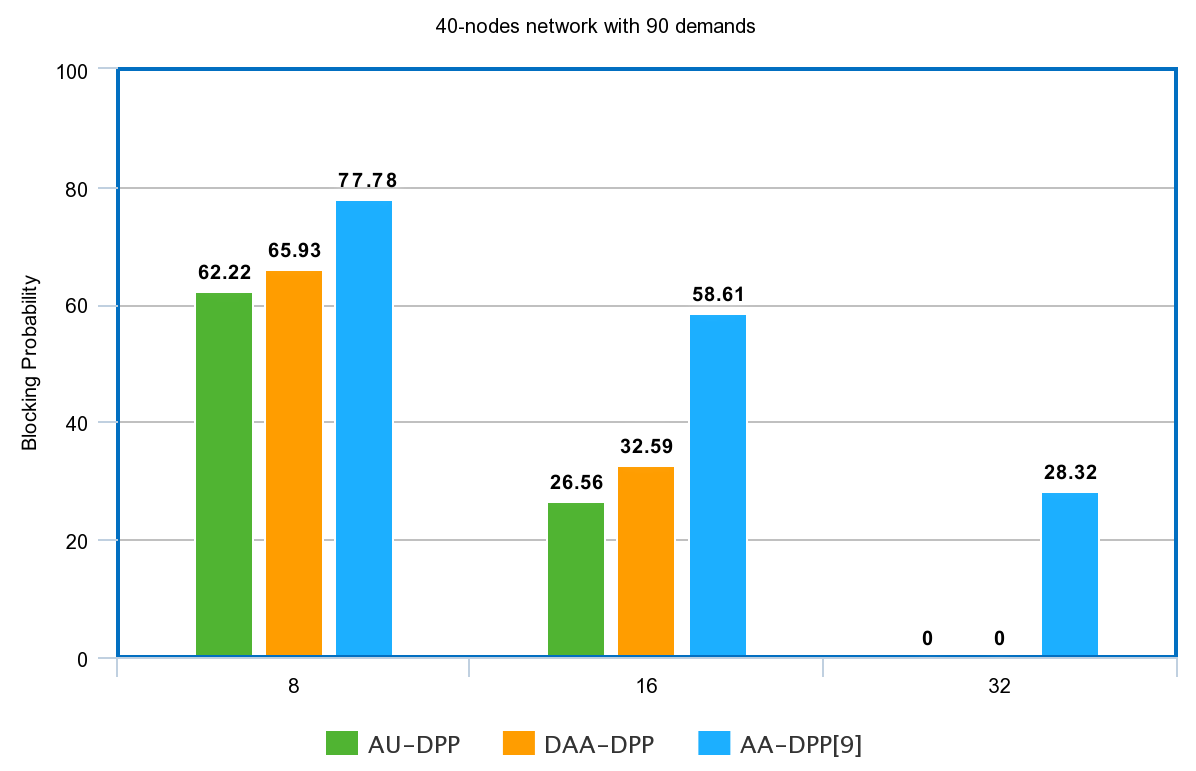
\includegraphics[scale= 0.3]{img/chart2.png}
		\caption{{\em  Comparison of blocking probabilities with different number of channels }}
		%	\label{triangleQG}
		\end{figure}
		
Fig. 4.6 shows that the blocking probability of the AA-DPP approach exceeds the blocking probability of the proposed approached tested with different number of channels per fiber.

\chapter{Conclusion and Future Work}

\section{Conclusion}

In this thesis, we propose an integer linear program (ILP) formulation approach to address the attack-aware RWA problem for dynamic traffic model \cite{papageorgiou1990dynamic}, using dedicated path protection (DPP) \cite{wiki:PP} in WDM optical networks. We have used the dedication path protection scheme to secure the transmission of data in case an attack occurs in any part of the network. The main objective of the ILP formulation is to maximize the number of successful requests in the network, while minimizing the path lengths of all the primary and backup paths.
The proposed approach finds a feasible route and channel for the primary and backup lightpath of each demand, such that both primary and backup lightpaths are not vulnerable to attack by the same existing lightpath. This helps in reducing the effects of various attacks, namely in-band jamming attacks, and out-of-band jamming attacks.

We have used different sizes of networks (14, 20, and 40 nodes) and the different number of channels per fiber for each network size. We have compared our model with the AA-DPP[9] and attack unaware RWA for the dynamic traffic model using dedicated path protection. The proposed ILP uses an attack model where the attacking signal can affect the first adjacent channel only. Our experimental results indicate that, the blocking probability associated with DAA-RWA results in blocking probabilites that are only slightly higher than attack unaware model. We have also compared our results to an existing attack-aware model using DPP, where the attacking signal can affect all the channels of the fiber. We found that the blocking probability of our proposed ILP is lower than the blocking probability of the approach used in [9].


\section{Future Work}

In order obtain a fully secure and robust RWA, we can use shared path protection technique with our proposed attack aware ILP approach. In case of the dedicated path protection, a separate backup lightpath is assigned for each primary lightpath in the optical network. The backup lightpath is utilized only if there is an attack on the primary lightpath otherwise it remains unused. Hence, we may consider studying the performance of the WDM networks using the shared path protection approach, which typically leads to better utilization of available resources. Moreover, to handle larger network instances, a fast heuristic approach using shared path protection may be proposed to accommodate a large number of demands with faster execution times.

\bibliographystyle{abbrv}
\bibliography{references}

\cleardoublepage
\thispagestyle{plain}
\addcontentsline{toc}{chapter}{VITA AUCTORIS}
\begin{table}[htbp]
	\begin{tabular}{p{0.3\linewidth}p{0.65\linewidth}}
		\\
		\\
		\\
		\\
		\\
		\\
		\multirow{2}{*}
		{\Huge\bfseries VITA AUCTORIS} \\
		\\
		\\
		\\
		NAME: & Kamaljeet Singh Gill \\
		\\
		PLACE OF BIRTH: & Delhi, India. \\
		\\
		EDUCATION: & Bachelor of Technology in Computer Science, Punjab Technical University, Punjab, India, 2015.
		\vskip1em
		
		\vskip1em
		Master of Science in Computer Science, University of Windsor, Windsor, Ontario, Canada, 2018.\\
	\end{tabular}
\end{table}

\end{document}
